\documentclass[11pt]{article}
\usepackage{lmodern}
\usepackage[utf8]{inputenc}
\usepackage{braket}
\usepackage{amsmath}
\usepackage[T1]{fontenc}
\usepackage{tgpagella}
\usepackage{graphicx}
\usepackage{caption}
\usepackage{subcaption}
\usepackage[utf8]{inputenc}
\usepackage{amssymb}
\usepackage[dvipsnames]{xcolor}
\usepackage{graphicx}
\usepackage{caption}
\usepackage{float}
\usepackage{tikz}
\usetikzlibrary{lindenmayersystems}
\usepackage[usestackEOL]{stackengine}
\newtheorem{theorem}{Theorem}[section]
\usepackage{appendix}
\usepackage{biblatex}
\usepackage[capitalise]{cleveref}
% \addbibresource{biblio.bib}
\usepackage{imakeidx}
\usetikzlibrary{calc}
\usepackage[normalem]{ulem}


% BOXES COMMANDS
    \newcommand*{\boxcolor}{RubineRed}
    \makeatletter
    \renewcommand{\boxed}[1]{\textcolor{\boxcolor}{%
    \tikz[baseline={([yshift=-1ex]current bounding box.center)}] \node [rectangle, minimum width=1ex,rounded corners,draw] {\normalcolor\m@th$\displaystyle#1$};}}
    \makeatother

% NOTES COMMANDS
    \usepackage{todonotes}
    \newcommand{\todonew}[2][]{\todo[linecolor=green!70!white, backgroundcolor=SpringGreen,
    bordercolor=green!70!white, textcolor=violet]{#2}}
    \newcommand{\tododo}[2][]{\todo[linecolor=green!70!white, backgroundcolor=blue!20!white,
    bordercolor=green!70!white, textcolor=violet]{#2}}
    \newcommand{\todoquestions}[2][]{\todo[linecolor=green!70!white, backgroundcolor=orange!20!white,
    bordercolor=green!70!white, textcolor=violet]{#2}}

% COLORS COMMANDS

\newcommand{\important}[1]{\textcolor{OrangeRed}{\bf{#1}}}

\linespread{1.2}

    \usepackage{geometry}
    \geometry{
     a4paper,
     left=25mm,
     right=25mm,
     top=25mm,
     bottom=30mm,
     }

\title{Coupled Local Supervised Learning Notes}
\author{Monica Conte}
\date{March 2023}

\begin{document}
\captionsetup{width=0.85\textwidth}

\maketitle

\renewcommand{\abstractname}{}
\begin{abstract}
    In this document I review the theory on \textit{Coupled Local Supervised Learning} (CLSL) as explained in \cite{} and applied in \cite{}. This method constitutes a novel approach in the design of materials.

\end{abstract}

\tableofcontents


\newpage

\section{Intro}

As opposed to materials designed with particular sets of functions, CLSL approach allows to create systems that don't possess explicit infomration about the desired functionality but physically adapts to applied forces and develop the ability to perform tasks. This method belongs to a class of strategies based on learning, where systems can adjust or be adjusted microscopically in response to training set to develop desired functionalities. Until recently, such idea was primarily applied in the context of non-physical networks, like artificial neural networks (ANN).

There are two types of learning. 
\begin{itemize}
\item \textbf{Global Learning} involves the minimization of a global function and the subsequent \textit{tuning} of the leaning degrees of freedom. \important{An external intervention at microscopic level is required.} 
\item In \textbf{Local Lerning} the evolution is \important{autonomous and requires no external designer} for the evaluation of the current state and subsequent modification. This is particularly useful in physical systems since their microscopical elements do not perform computations and do not encode a priori infomration about the desired functionality. 
\end{itemize}

CLSL implements local learning on physical netwroks with the aim of training it to achieve desired responses on \textit{target nodes} as a response to external constraints applied to \textit{source nodes}. The method is inspired by \textit{contrastive learning} and by the strategy of \textit{equilibrium propagation}. In the paper, it is applied to two types of physical systems, a flow network and an elastic network. Experimental issues are finally taken into consideration and the theory of the method is modified accordingly. 

\newpage

\section{ANN framework}

The building blocks of ANN are \textit{neurons}. They are elements that take inputs and produce outputs by performing some mathematical operations on the inputs. \cref{fig:neuron} shows a neuron with two inputs $x_1$ and $x_2$. The output depends on the inputs, the wieght and the bias. Training a neuron means modifying the wieghts in such a way that it outputs a desired value.
\begin{figure}[h]
    \centering
    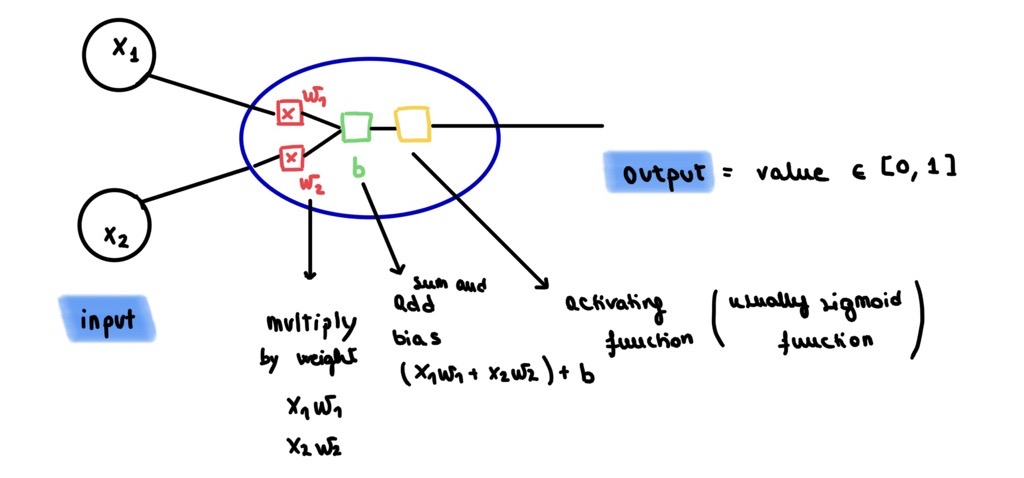
\includegraphics[width=0.75\columnwidth]{figures_tex/neuron.png}
\caption{Two inputs ($x_1$ and $x_2$) neuron. Blue circle contains the operations perfomred in a neuron: \textcolor{red}{\textbf{multiply inputs to wieghts}} associated to the links, \textcolor{LimeGreen}{\textbf{sum inputs and add a bias $b$}}, \textcolor{Dandelion}{\textbf{apply an activating function}}. The outcome is a value belonging to $[0,1]$.}
    \label{fig:neuron}
\end{figure} 

\textit{Neural networks} are structures made of many neurons. These neurons are organized in layers, an example in \cref{fig:neural_ntw}. There are three types of layers: input layer, hidden layers and output layers. Input layers read the inputs, operations are perfomed in the hidden layer and output is generated in ouput layer. Hence, a neural network can be seen as a set of \textit{nodes} (the neurons) connected by \textit{edges} (the links with wieghts).
Given an input, each neuron in each layer performs coputations and gives output that are inputs for the follwoing neuron. This process of proceeding from the inputs to the outputs is called \textbf{feedforward}.
\begin{figure}[h]
    \centering
    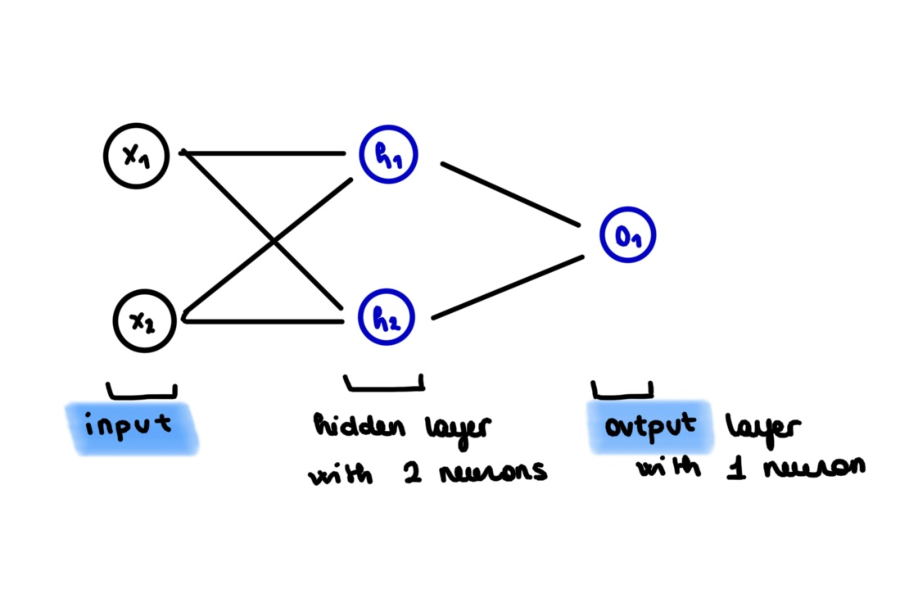
\includegraphics[width=0.6\columnwidth]{figures_tex/neural_ntw.pdf}
    \caption{Example of a neural network: a structure made of neurons organized in layers.}
    \label{fig:neural_ntw}
\end{figure} 

A neural network needs \textit{training} in order to be able to perform a task. The standard way to train a network is by using a \textit{loss function}, which quantifies how good the output of the network is compared to the desired output. Often, the mean-squared error (MSE) is used
\[
\text{MSE} = \frac{1}{N} \sum_{i=1}^{N} (y_{\text{desired}} - y_{\text{predicted}})^2    
\]
where the sum is take over the training samples and $y$ indicates the value of the output in a specific neuron. From this simple formula we can already uderstand that a \important{smaller error implies a better prediction}. 

The trainig method proceeds in changing the weights in the network in the direction of the minimization of the loss funtion. It is therefore useful to denote as $L(\mathbf{w})$ the loss function as a function of the set of wieghts $\mathbf{w}$. In oerder to understand how the loss function changes when the weight are modified, we consdier the derivative of the loss function with respect to the weights. Let us take for example the first wieght $w_1$, the derivative $\partial L/\partial w_1$ is found by applying the chain rule
\[
\frac{\partial L}{\partial w_1} = \frac{\partial L}{\partial y_{\text{predicted}}} \frac{\partial y_{\text{predicted}}}{\partial w_1}    
\]
which is applied again to the second therm on the RHS following a path in the neural network which traces back to the location of the weight $w_1$. This procedure is called \textbf{backpropagation} since it acconts in propagating back the error in the network and identify the biggest sources of error. 

Once the derivative of the loss function is calculated, one needst o find a way of optimizing the netwrok accordingly. A possible way of minimizing the loss function is by using \textbf{gradient descent} method. The weights are updated as follows:
\[
w \ \ \rightarrow w - \eta \frac{\partial L}{\partial w}    
\]
and the logic behind is that it changes the wiehgt towards the direction of descent. In fact, a positive derivative means that a positive increase of the wieght increases the loss function, from which a negative sign in front of the term. Viceversa for the negative sign. 

The training proceeds in steps and in each step the weights are optimized to decrease the error. There are many training samples in a dataset and a common training procedure randomly selects, at each step, one of the samples in the set and performs gradient descent. This procedure is called \textbf{stochastic gradient descent}.

\newpage

\section{CLSL framework}

We now consider a physical neural network (PNN). It is, again, a strucutre made of nodes and edges but, as opposed to ANN, they are not organized in layers and in principle there is no fixed patterns. However, just like an ANN, we divide the nodes in \textit{source nodes}, \textit{hidden nodes} and \textit{target nodes}. A generic PNN is shown in \cref{fig:general_graph}. These elements assume values of physical qunatities and can be realized in real life. For example, in electric netwroks, the nodes assume vlaue of potential and the edges of resistances.
\begin{figure}[h]
    \centering
    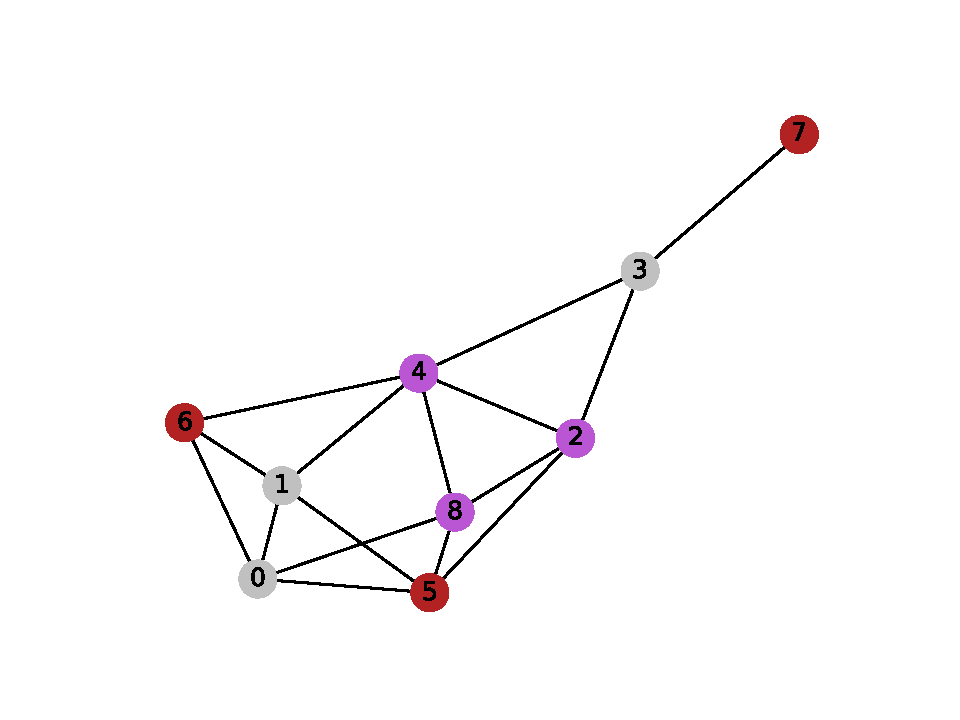
\includegraphics[width=0.6\columnwidth]{figures_tex/general_graph.pdf}
    \caption{Example of a generic PNN. $5,6,7$ red dots denote input nodes, $0,1,3$ gray nodes denote hidden nodes and $2,4,8$ purple nodes denote target nodes.}
    \label{fig:general_graph}
\end{figure} 
The training goal here is to train the netwrok to give desired outputs in the output nodes given cerain inputs at the source nodes, just like in the ANN.

In a PNN, the values on the nodes are produced by minimizing an \textit{energy function}, as opposed to the feedforward procedure of ANN. For example, in electric networks the function minmized is the power dissipated in the resistances, which corresponds to satisfying Kichoff's law on current in the circuit of nodes and resistances (see Appendix (?)), i.e. conservation of charge. In flow networks, minimization of power means conservation of flow (?).

\subsection{General formulation of the method}

Let us consdier a network with nodes $\mu$ and indeces $j$. The \textit{physical degrees of freedom} (pof) belong to the set of variables $\{ x_{\mu}\}$. The \textit{learning degrees of freedom} (lof) belong to the set $w_j$ and play the roles of wieghts connecting the nodes. Given an initial condition $x_{\mu}(t=0)$ (part of the $x_{\mu}$ in the set given) and a set of weights, the physical degrees of freedom evolve to a steady state tha minimizes a \textit{physical cost function} $E(x_{\mu};w_j)$. Note that both $\{ x_{\mu} \}$ and $E$ depend on $\{ w_j\}$.

Inspired by \textit{contrastive Hebbian learning} (CHL) [], one considers two states of the network. A \textit{free state} $x_{\mu}^{F}$ in which the source nodes $x_S$ are constrained while the target $x_T^F$ and hidden $x_H^F$ equilibrate to the steady state. A \textit{clamped state} $x_{\mu}^{C}$ in which the source $x_S$ and the target $x_T^C$ nodes are constrained while only the hidden nodes $x_H^C$ equilibrate to the steady state. In the clampd state, the target nodes are nudged by an \textit{external supervisor} towards the desired $X_T$ values of outputs
\[
x_T^{C} = x_{T}^F + \eta \left[ X_T - x_{T}^{F} \right] 
\] 
with $\eta \ll 1$. In contrast with CHL, the nudge parameter is small, which fixes the problem of free and clamped state reaching two different local minima of the energy function.

The authors propose the following updating rule for the lof:
\[
\dot{\mathbf{w}} = \alpha \eta^{-1} \partial_{\mathbf{w}} \left\{ E(x_S, x_{H}^{F}, x_{T}^{F}) - E(x_S, x_{H}^{C}, x_{T}^{C}) \right\}   
\]

\begin{itemize}
    \item $\boldsymbol{\alpha}$ is a scalar \bf{learning rate}
    \item $\boldsymbol{\eta}$ is the \bf{nudging aplitude}.
\end{itemize}

% which corresponds to performing a gradient descent on the energy function with respect to the wiehgts. This means that the wieghts are updated towards a local minima of the energy function. 
The motivation behind this rule comes from the fact that we consdier a \important{physical} network, where generally one can partition the total energy $E$ as a sum over edegs $E = \sum_{j}E_{j}(x_{\mu}(j);w_j)$ of energies $E_j$ that only depend on the pof on the nodes that connect the edge $j$. Therefore, the learning rule is \important{local}. But does this rule effectively trainst the network? The autors actually show (Appendix A in paper) that this updating scheme minimizes an \textit{effective cost function} that is not identical to the standard cost function but shares important features with it. They argue that minimizing the effective function mimics the minimization of a standard cost function. From how well the networks are trained, they observe that this affirmation is plausible. The CLSL approach share many similarities with Equilibrium Propagation(EP) \cite{} and the learning rule has the same form. However, in EP the learning rule minimizes an actual cost function.

Summarizing, the learning approach involves the minimization of an energy function and the implementation of the proposed updating rule. The former is motivated by physical plausability and the latter by inspiration from EP. A comparison with minimization of an actual cost function is needed. \textcolor{Orchid}{They say EB is a type of contrastive learning.}

\subsection{Application to Electrical Netwroks}

The framework above can be applied in the context of an electrical network, in which nodes are connected by \textit{variable resistors}. When input voltages are applied at the source nodes $V_{S}$, the voltages at the output $V_{O}$ and hidden $V_{H}$ nodes are determined such that the total power dissipated by the resistances $\mathcal{P}$ is minimized
\[
\mathcal{P}  = \frac{1}{2} \sum_{j} \frac{\Delta V_j^2}{R_j}   
\]
where $j$ runs over the resistances $R_j$ and $\Delta V_j$ is the potential difference between the nodes that the resistance links.

We define the two types of states as above. In the free state the source nodes $V^{F}_{S}$ are constrained, while $V^{F}_{H}$ and $V^{F}_{T}$ are determined by minimizing $\mathcal{P}$. In the clamped state, the source nodes $V^{F}_{C}$ are fixed to the source values, the target nodes are clamped 
\[
V^{C}_{T} = V^{F}_{C} + \eta \left( V^{D} - V^{F}_{C} \right)   
\] 
towards the desired output voltages $V^D$, while the hidden nodes are left to minimize $\mathcal{P}$. The parameter $0 < \eta \le 1$ quanitifies the importance of the nudge.

The final goal is deriver the desired output $V^{D}$ in the target nodes. To do so, the network gets optimized by updating the values of the resistances following a certain \textit{learning rule}. The adaptation of the learning tule of CLSL in the context of electrical circuit would lead to 
\begin{equation}
\boxed{\dot{R}_j = \frac{\alpha}{2\eta R_{j}^2} \left[ \left( \Delta V_{j}^{C}\right)^2 - \left( \Delta V_{j}^{F}\right)^2 \right] }
\label{eq:cont_rul_res}   
\end{equation}
where $R_{j}$ is the selected resistance to update, $\Delta V_{j}^{C}$ is the potential difference between the nodes that it connects in the clamped state and $\Delta V_{j}^{F}$ the difference in the free state. In the paper [dillavou] they define
\[
\gamma = \frac{\alpha}{2\eta}
\]
as the learning rate.

In the experiment, they have discrete resistors and the rule above gets approximated with the following 
\begin{equation}
\boxed{\dot{R}_j = \begin{cases} 
    +\delta R & \text{if} \ |\Delta V^{C}_{j}|>|\Delta V^{F}_{j}| \\
    -\delta R & \text{otherwise}
 \end{cases}}
\label{eq:disc_rul_res}
\end{equation}
which consists in taking the sign of \cref{eq:cont_rul_res} and multipy it by the value $\delta R$.

\subsection{Comparison with standard methods}

\end{document}